% higgs_composite_qg.tex (generated; edit src/higgs_composite_qg.template.tex) -- Regular Article for Physical Review D (REVTeX 4.2), revised hypotheses; second version of the
% text (22 November 2026), rewritten at the author's request to be self-contained and friendlier to a student reader.
% PROJECT spacetimes, folder Revision_SM_Higgs/paper_prd.
% This file is generated from src/higgs_composite_qg.template.tex by scripts/build_paper.py, which inserts every number
% that a program computes, from the data files and the reports of the checks of the folder data/ (the bounds of the
% agreement of two computations rounded up), and every value of the worked examples of Sec. II from data/sh_examples*.csv
% (the placeholders EX:<name> in double braces; EX_TABLE_CHARGES is the table of the eight spinor charges, from
% data/sh_examples_charges.csv).  Typed in the template are only the parameters of the model and of the numerical method,
% mathematical constants, the quantum numbers that the hypotheses assign, the definitions of the algebra, and measured
% values of the Standard Model with their references.
% Build:  python3 paper_prd/scripts/build_paper.py   (writes higgs_composite_qg.tex and runs pdflatex and bibtex)
\documentclass[aps,prd,twocolumn,superscriptaddress,nofootinbib,floatfix,longbibliography]{revtex4-2}
\usepackage{amsmath,amssymb}
\usepackage{graphicx}
\usepackage{bm}
\usepackage[colorlinks=true,linkcolor=blue,citecolor=blue,urlcolor=blue]{hyperref}
\hypersetup{pdftitle={Higgs as a Composite, and Quantum Gravity},pdfauthor={Patrick Lee Nash}}

% the suffixes of the symbols of PROJECT spacetimes: LL (the Lorentz super-loop and its fields, Sec. II), SF (the
% superfluid of the earlier hypotheses) and SH (the objects of the revised hypotheses of this paper)
\newcommand{\LL}{{\rm LL}}
\newcommand{\SF}{{\rm SF}}
\newcommand{\SH}{{\rm SH}}
\newcommand{\tr}{\mathrm{tr}}
\newcommand{\e}[1]{\mathbf e_{#1}}

\begin{document}

\title{Higgs as a Composite, and Quantum Gravity}

\author{Patrick Lee Nash, Ph.D.}
\affiliation{PROJECT spacetimes}

\date{November 22, 2026}

\begin{abstract}
Can the Higgs field be a condensate of pairs of fermions, as the state of a superconductor is a condensate of pairs of
electrons? We study this question in a model built on an algebraic structure, the Lorentz super-loop: the bi-octonions
of unit norm, a Moufang loop (a set with a product that has an identity and inverses but is not associative). It
contains the Lorentz group $SL(2,\mathbb C)$ and eight spinor charges, which are carried by an isodoublet $\Psi$ of
Dirac spinors. We first show, with worked examples, how these objects arise, and why pairs of two members of $\Psi$
form isospin triplets, so that a condensate of $\Psi$ alone cannot be the Higgs doublet of the Standard Model. We then
give $\Psi$ the hypercharge $\frac14$, add two singlet Dirac fields $\chi$ and $\chi'$ with the hypercharges $\frac14$
and $-\frac34$, and let a contact interaction bind a member of $\Psi$ to a singlet in a pair of spin zero. The two pair
fields form a bidoublet of $SU(2)_L\times SU(2)_R$ (a $2\times2$ matrix of fields on which the two groups act from the
left and from the right) with the quantum numbers of two Higgs doublets. In five mean-field methods (Hubbard-Stratonovich
with three decouplings, Kohn-Sham, and Cornwall-Jackiw-Tomboulis) the ground state is the custodial vacuum, which keeps
the symmetry that protects the ratio of the $W$ and $Z$ masses: it breaks $SU(2)_L\times U(1)_Y$ to the $U(1)$ of the electric charge, keeps the photon massless
and gives $\rho=1$. Setting its scale to $v=246.22$~GeV puts the momentum cutoff at 2.2\mbox{--}2.4~TeV. The amplitude
mode, the oscillation of the size of the condensate and the candidate for the Higgs boson, is a composite scalar bound
below the threshold of two quasi-particles. Where only the pairing acts, the linear response has the closed form of the
theory of Bardeen, Cooper and Schrieffer and places the mode exactly at the pair self-energy (the gap parameter of
that theory): $M_H/v=7.967$,
16 times the measured $m_H/v=0.5082$, and over a scan of the coupling from 1.02 to 3 times its critical
value, with two masses of the fields, the ratio is at least \ensuremath{4.892}. A custodial triplet of massive scalars and
a Goldstone boson of the particle number come with it. The superfluid therefore has the quantum numbers of the Higgs
field and gives the $W$ and $Z$ bosons their masses, but in the mean field its amplitude mode is far too heavy. We
outline how gravitation will enter through E.~A.~Lord's gauge theory of the local change of spinor representation.
\end{abstract}

\maketitle

%=====================================================================================================================
\section{Introduction}
\label{sec:intro}

The particle discovered at the Large Hadron Collider in 2012~\cite{ATLAS2012,CMS2012} has, within uncertainties of a few
per cent, the couplings of the elementary Higgs boson of the Standard Model~\cite{ATLAS2022,CMS2022}. Whether the Higgs
field is elementary, or a composite of more fundamental fields, is nevertheless one of the oldest open questions about
it. The question has a familiar prototype in the physics of metals. In a superconductor the electrons bind into Cooper
pairs, and below a critical temperature a macroscopic number of pairs occupy the same pair state: they form a
\emph{condensate}. The condensate gives the photon a mass inside the material (this is why a magnetic field is expelled,
the Meissner effect), and it costs a finite energy, the \emph{gap}, to break a pair. Bardeen, Cooper and Schrieffer (BCS)
explained all of this with an attraction between the electrons and no elementary scalar field at all~\cite{BCS1957}.
In the Standard Model the Higgs field plays the same role for the $W$ and $Z$ bosons: its constant value in the vacuum
makes them massive. The idea of a composite Higgs field is that this constant value, too, is a condensate of pairs.

Nambu and Jona-Lasinio turned the BCS idea into a model of particle physics~\cite{NJL1961}: a contact interaction of
four fermion fields, above a critical strength, condenses the fermions, gives them a gap (a mass), and produces a
composite scalar particle whose mass is tied to that gap. Later proposals range from technicolor~\cite{Weinberg1976,
Susskind1979} and the condensation of the top quark~\cite{Miransky1989,BHL1990} to a Higgs boson that is a
pseudo-Goldstone boson of a strongly coupled sector (a light particle that comes with a slightly broken
symmetry)~\cite{KaplanGeorgi1984,Agashe2005}; the review of Hill and
Simmons~\cite{HillSimmons2003} describes their dynamics.

This paper asks the same question for a definite set of fermion fields, those of the \emph{Lorentz super-loop}. The
bi-octonions of unit norm, the elements of a sixteen-dimensional algebra of numbers, form a \emph{Moufang loop}: a set
with a product that has an identity element and inverses, like a group, but whose product is not associative. The author
has called this loop the Lorentz super-loop and has shown that it contains the Lorentz group $SL(2,\mathbb C)$, and
beside it eight \emph{spinor charges}, quantities that turn under rotations as spin $\frac12$ does~\cite{Nash2026}. The
fields that carry the spinor charges form an isodoublet $\Psi_\LL$ of Dirac spinors, and an attraction between them
produces a superfluid of pairs of spin zero. Section~\ref{sec:algebra} builds all of these objects from the beginning,
with a worked example of each, so that this paper can be read without any other.

That superfluid cannot be the Higgs field. A pair of two members of one isodoublet has isospin 1 (Sec.~\ref{sec:algebra}),
while the Higgs field has isospin $\frac12$. The present paper therefore changes the hypotheses. Two singlet Dirac
fields are added, the hypercharges are chosen so that a pair of a member of $\Psi_\LL$ and a singlet has exactly the
quantum numbers of the Higgs doublet, and the attraction acts in those pairs (Sec.~\ref{sec:model}). We then ask, in five
mean-field methods: does the superfluid form? Which symmetries does it break? Which gauge bosons does it make massive,
and with what ratio of the masses of the $W$ and $Z$ bosons? How heavy is its amplitude mode, the particle that would
be the Higgs boson? And how does that mode move in time?

The answers are as follows. In every method the ground state is the \emph{custodial superfluid}, a condensate that
keeps the custodial symmetry of the Standard Model (Sec.~\ref{sec:model}), the symmetry that protects the ratio of the
masses of the $W$ and $Z$ bosons: it breaks the symmetries exactly as the Standard Model does, keeps the photon massless and gives the measured ratio of the $W$ and $Z$ masses
($\rho=1$, Sec.~\ref{sec:gauge}). With its scale set to $v=246.22$~GeV, the $W$ and $Z$ bosons have their measured
masses at tree level. The two pair fields carry the scalars of two Higgs doublets. The amplitude mode is a composite
scalar, but it lies near the energy that breaks a pair, and the scale of the breaking is small compared with that
energy: the ratio $M_H/v$ is about sixteen times its measured value. Within the mean field, the superfluid is the Higgs
field of the Standard Model in its quantum numbers and in the masses it gives the gauge bosons, but not in the mass of
its own boson.

The gauge group of the model contains $SL(2,\mathbb C)$ as a factor, with a Lorentz connection that is a pure gauge on
the flat space-time of this paper. E.~A.~Lord showed in 1971 that making the local change of representation of the
two-component spinors a Yang-Mills gauge group leads, with the necessary auxiliary fields, to a self-interacting field
of spin two identical with Einstein's gravitation~\cite{Lord1971}. Section~\ref{sec:gravity} outlines how that
construction will make the gravitational sector of this model; it is a program, and no part of it is computed here.

\paragraph*{How to read this paper.} We assume what a first-year graduate student knows: special relativity, the Dirac
equation, second quantization, and the elements of group theory (groups, their representations, Lie algebras). Every
other notion is defined where it is first used, and most come with a small example whose numbers can be checked by
hand. Symbols carry a suffix that says where they come from: LL for the objects of the Lorentz super-loop and its fields
(Sec.~\ref{sec:algebra}), SF for the superfluid of those fields, and SH for the objects of the model of this paper
(Sec.~\ref{sec:model}); a suffix is dropped where nothing else uses the same letter. Every number of the paper is
produced by programs in Rust; independent programs in Python check the key results with their own engines, and scripts
in the Wolfram Language check the group theory and the closed forms in exact arithmetic. The Supplemental
Material~\cite{SM} gives the longer derivations, the checks and the data; nothing in the text needs it.

%=====================================================================================================================
\section{The algebra behind the model}
\label{sec:algebra}

This section explains, from the beginning, the algebraic objects from which the fields of the model come: the
octonions, the bi-octonions and their loop, the Lorentz group inside it, the eight spinor charges and the fields that
carry them, and the superfluid that those fields form. It follows Ref.~\cite{Nash2026}, but everything needed here is
stated and derived here. Each object comes with a worked example. The numbers of the examples of
Secs.~\ref{sec:oct}--\ref{sec:spinors} are exact rationals, those of Sec.~\ref{sec:sf} come from one-dimensional
integrals. A Rust program computes all of them, a Python program recomputes every one (the algebra in exact rational
arithmetic), and a Wolfram Language script derives the general identities behind them symbolically. A reader who knows
the octonions can skim Secs.~\ref{sec:oct} and~\ref{sec:bioct}.

\subsection{Octonions, and a loop that is not a group}
\label{sec:oct}

The \emph{quaternions} are the numbers $a_0\e0+a_1\e1+a_2\e2+a_3\e3$ with real $a_p$, where $\e0=1$ and the three
imaginary units obey
\begin{equation}
\e1^2=\e2^2=\e3^2=-\e0,\qquad \e1\e2=-\e2\e1=\e3
\label{eq:quat}
\end{equation}
and the cyclic permutations ($\e2\e3=\e1$, $\e3\e1=\e2$). Their product is associative but not commutative. The
\emph{octonions} double them. Write an octonion as a pair of quaternions, $\mathbf x=\mathbf a+\mathbf b\,\e4$, and
multiply by the rule of Cayley and Dickson,
\begin{equation}
(\mathbf a+\mathbf b\,\e4)(\mathbf c+\mathbf d\,\e4)=(\mathbf a\mathbf c-\bar{\mathbf d}\mathbf b)+(\mathbf d\mathbf a
+\mathbf b\bar{\mathbf c})\,\e4 ,
\label{eq:cd}
\end{equation}
where the bar changes the signs of the coefficients of $\e1$, $\e2$, $\e3$. The eight units are $\e0,\dots,\e3$, $\e4$,
and $\e5=\e1\e4$, $\e6=\e2\e4$, $\e7=\e3\e4$. The product of any two units is again a unit, up to a sign. For example,
\begin{equation}
\e1\e2=\e{3},\qquad \e2\e1=-\e{3},
\end{equation}
so the product is not commutative, and
\begin{equation}
(\e1\e2)\e4=\e{7},\qquad \e1(\e2\e4)=-\e{7},
\label{eq:nonassoc}
\end{equation}
so it is not associative either. The \emph{associator} $[\mathbf x,\mathbf y,\mathbf z]=(\mathbf x\mathbf y)\mathbf
z-\mathbf x(\mathbf y\mathbf z)$ measures the failure; here $[\e1,\e2,\e4]=2\e{7}$. The octonions keep
a weaker property: the associator vanishes whenever two of its arguments are equal, so that any two octonions generate
an associative subalgebra (the algebra is called \emph{alternative}). And the \emph{norm}
$N(\mathbf x)=\sum_pa_p^2$ (the sum of the squares of the eight coefficients) is multiplicative,
$N(\mathbf x\mathbf y)=N(\mathbf x)N(\mathbf y)$, with $\mathbf x\bar{\mathbf x}=N(\mathbf x)\,\e0$, where now the bar
changes the signs of the coefficients of $\e1,\dots,\e7$.

Associativity is what turns a set with a product into a group. Without it one has a \emph{loop}: a set with a product,
an identity element, and unique solutions $\mathbf x$ of the equations $\mathbf w\mathbf x=\mathbf y$ and $\mathbf
x\mathbf w=\mathbf y$. A loop that obeys the three \emph{Moufang identities}
\begin{equation}
\begin{gathered}
\mathbf z(\mathbf x(\mathbf z\mathbf y))=((\mathbf z\mathbf x)\mathbf z)\mathbf y,\qquad
((\mathbf y\mathbf z)\mathbf x)\mathbf z=\mathbf y(\mathbf z(\mathbf x\mathbf z)),\\
(\mathbf z\mathbf x)(\mathbf y\mathbf z)=(\mathbf z(\mathbf x\mathbf y))\mathbf z
\end{gathered}
\label{eq:moufang}
\end{equation}
is a \emph{Moufang loop}~\cite{Moufang1935}; every group is one, but not every Moufang loop is a group. The simplest
example that is not a group is close at hand: the sixteen elements $\pm\e0,\dots,\pm\e7$, with the product of the
units. It is a loop with 16 elements; the identities~(\ref{eq:moufang}) hold for all 4096
ordered triples of its elements (a program finds 0 failures), yet 1344 of 4096 triples are not
associative, Eq.~(\ref{eq:nonassoc}) being one of them, and 168 of 256 ordered pairs do not commute.
The octonions of norm 1 form a larger Moufang loop, the seven-sphere. With $\mathbf x=\tfrac{3}{5}\e{0}+\tfrac{4}{5}\e{1}$,
$\mathbf y=\tfrac{3}{5}\e{2}+\tfrac{4}{5}\e{4}$ and $\mathbf z=\tfrac{1}{3}\e{0}+\tfrac{2}{3}\e{3}+\tfrac{2}{3}\e{6}$, three octonions of norm 1, the product $\mathbf x\mathbf y=
\tfrac{9}{25}\e{2}+\tfrac{12}{25}\e{3}+\tfrac{12}{25}\e{4}+\tfrac{16}{25}\e{5}$ again has norm 1, while $(\mathbf x\mathbf y)\mathbf z$ and $\mathbf x(\mathbf y\mathbf z)$ differ by the
associator $-\tfrac{64}{75}\e{3}+\tfrac{16}{25}\e{5}+\tfrac{64}{75}\e{6}$.

\subsection{Bi-octonions and the Lorentz super-loop}
\label{sec:bioct}

Allow complex coefficients: $\mathbf x=\sum_{p=0}^7\xi_p\,\e p$ with $\xi_p\in\mathbb C$. The imaginary unit $i$ of the
coefficients commutes with every unit $\e p$; it is not one of them. These \emph{bi-octonions} form an algebra of
real dimension 16 with the same product~(\ref{eq:cd}), now applied to \emph{bi-quaternions} (quaternions with complex
coefficients). The norm $N(\mathbf x)=\sum_p\xi_p^2$ is now a complex number, still multiplicative. The bi-octonions of
norm 1,
\begin{equation}
\mathbb L_\LL=\{\mathbf w:\ N(\mathbf w)=1\},
\label{eq:loop}
\end{equation}
form a Moufang loop. The product of two of them has norm 1, $\e0$ is the identity, and $\bar{\mathbf w}$ is the inverse
of $\mathbf w$, since $\mathbf w\bar{\mathbf w}=N(\mathbf w)\,\e0=\e0$. The equation $\mathbf w\mathbf x=\mathbf y$ has the
unique solution $\mathbf x=\bar{\mathbf w}\mathbf y$: the two elements $\mathbf w$ and $\mathbf y$ generate an associative
subalgebra (Sec.~\ref{sec:oct}), which contains $\bar{\mathbf w}=2\xi_0\e0-\mathbf w$, so $\mathbf w(\bar{\mathbf
w}\mathbf y)=(\mathbf w\bar{\mathbf w})\mathbf y=\mathbf y$, and in the same way $\mathbf w\mathbf x=\mathbf y$ gives
$\mathbf x=\bar{\mathbf w}\mathbf y$. The Moufang identities~(\ref{eq:moufang}) hold in every alternative
algebra~\cite{Schafer1966}, so they hold in $\mathbb L_\LL$. The author calls this loop the \emph{Lorentz
super-loop}~\cite{Nash2026}, for the reason that the next two subsections show: it contains the Lorentz group, and beside
it charges of spin $\frac12$. It is a smooth manifold of complex dimension 7 (one complex equation in $\mathbb C^8$). For
example, $\mathbf w=\tfrac{3}{4}\e{0}+\tfrac{9}{20}i\e{3}+\e{4}+\tfrac{3}{5}i\e{7}$ has norm 1; its inverse is $\bar{\mathbf
w}=\tfrac{3}{4}\e{0}-\tfrac{9}{20}i\e{3}-\e{4}-\tfrac{3}{5}i\e{7}$, and the solution of $\mathbf w\mathbf x=\e5$ is $\mathbf x=\bar{\mathbf w}\e5=-\e{1}+\tfrac{3}{5}i\e{2}+\tfrac{3}{4}\e{5}+\tfrac{9}{20}i\e{6}$.

\subsection{Space-time and the Lorentz group inside the loop}
\label{sec:lorentz}

The bi-quaternions of norm 1 are a subset of the loop that \emph{is} a group, because the product of bi-quaternions is
associative. The map
\begin{equation}
M_\LL(\e0)=\sigma_0,\qquad M_\LL(\e j)=-i\sigma_j\quad(j=1,2,3),
\label{eq:Mmap}
\end{equation}
with the Pauli matrices $\sigma_j$ and the unit matrix $\sigma_0$, extended complex-linearly, turns every bi-quaternion
into a complex $2\times2$ matrix and every product into the product of matrices, and the norm becomes the determinant.
The unit bi-quaternions are therefore the group $SL(2,\mathbb C)$ of complex $2\times2$ matrices of determinant 1, which is
the double cover of the Lorentz group: each Lorentz transformation corresponds to two matrices, $\pm M$.

Space-time enters as follows. A bi-quaternion $\mathbf x$ is \emph{Hermitian} if $\mathbf x^\dagger=\mathbf x$, where
the dagger is the bar combined with the complex conjugation of the coefficients. The Hermitian bi-quaternions are
exactly
\begin{equation}
\begin{gathered}
\mathbf x=x^0\e0+i\,(x^1\e1+x^2\e2+x^3\e3),\\
N(\mathbf x)=(x^0)^2-(x^1)^2-(x^2)^2-(x^3)^2,
\end{gathered}
\label{eq:m31}
\end{equation}
with real $x^\mu$: they are the points of Minkowski space, and their norm is the Minkowski interval with the metric
$\eta={\rm diag}(1,-1,-1,-1)$. We call this space M31. An element $\mathbf g$ of $SL(2,\mathbb C)$ acts on it by
$\mathbf x\mapsto\mathbf g\,\mathbf x\,\mathbf g^\dagger$, which keeps $\mathbf x$ Hermitian and its norm unchanged: it
is a Lorentz transformation. Here are two examples, with numbers chosen to be rational. The \emph{rotation} $\mathbf
g_{\rm rot}=\tfrac{3}{5}\e{0}+\tfrac{4}{5}\e{1}$ and the \emph{boost} $\mathbf g_{\rm boost}=\tfrac{5}{4}\e{0}+\tfrac{3}{4}i\e{3}$ have the matrices
\begin{equation}
M_\LL(\mathbf g_{\rm rot})=\begin{pmatrix}\tfrac{3}{5}&-\tfrac{4}{5}i\\-\tfrac{4}{5}i&\tfrac{3}{5}\end{pmatrix},\qquad M_\LL(\mathbf g_{\rm boost})=\begin{pmatrix}2&0\\0&\tfrac{1}{2}\end{pmatrix},
\label{eq:Mexamples}
\end{equation}
both of determinant 1. Written as $4\times4$ matrices $\mathsf L(\mathbf g)$ that act on the coordinates
$(x^0,x^1,x^2,x^3)$, the two Lorentz transformations are
\begin{equation}
\begin{gathered}
\mathsf L(\mathbf g_{\rm rot})=\begin{pmatrix}1&0&0&0\\0&1&0&0\\0&0&-\tfrac{7}{25}&-\tfrac{24}{25}\\0&0&\tfrac{24}{25}&-\tfrac{7}{25}\end{pmatrix},\\
\mathsf L(\mathbf g_{\rm boost})=\begin{pmatrix}\tfrac{17}{8}&0&0&\tfrac{15}{8}\\0&1&0&0\\0&0&1&0\\\tfrac{15}{8}&0&0&\tfrac{17}{8}\end{pmatrix}.
\end{gathered}
\label{eq:Lexamples}
\end{equation}
The first turns the plane of $x^2$ and $x^3$ about the $x^1$ axis by the angle whose cosine is $-\frac7{25}$. The second
moves the point at rest $(1,0,0,0)$ to $(\tfrac{17}{8},0,0,\tfrac{15}{8})$: it is a boost along $x^3$ with the Lorentz factor
$\frac{17}8$ and the velocity $\frac{15}{17}$.
The tangent directions of $SL(2,\mathbb C)$ at the identity are the imaginary bi-quaternions. With the rotation and boost
generators $J^j_\LL=\frac12\e j$ and $K^j_\LL=\frac12i\,\e j$, the commutators of Eq.~(\ref{eq:quat}) are those of the
Lie algebra of the Lorentz group; for example $[J^1_\LL,K^2_\LL]=K^3_\LL$. The unit $\e4$ supplies the
parity: conjugation by it, $\mathbf x\mapsto\e4\,\mathbf x\,\e4^{-1}=\bar{\mathbf x}$, reverses the three spatial
coordinates, so the point $(2,1,3,5)$ goes to $2\e{0}-i\e{1}-3i\e{2}-5i\e{3}$, i.e.\ to $(2,-1,-3,-5)$. (In a
non-associative product the expression $\e4\,\mathbf x\,\e4^{-1}$ needs no brackets, because the octonions are
\emph{flexible}, $(\mathbf a\mathbf b)\mathbf a=\mathbf a(\mathbf b\mathbf a)$, a consequence of alternativity.) No
bi-quaternion can do this: conjugation by an element of an associative algebra keeps the order of products,
$\mathbf g(\mathbf x\mathbf y)\mathbf g^{-1}=(\mathbf g\mathbf x\mathbf g^{-1})(\mathbf g\mathbf y\mathbf g^{-1})$, while
the bar reverses it, $\overline{\mathbf x\mathbf y}=\bar{\mathbf y}\,\bar{\mathbf x}$. In the loop, whose product is not
associative, the parity is conjugation by an element.

The loop contains much more than $SL(2,\mathbb C)$. The element $\mathbf s=\tfrac{3}{5}\e{0}+\tfrac{4}{5}\e{4}$ has norm 1 but is not a
bi-quaternion, and with it associativity fails even among elements of the loop:
$[\mathbf g_{\rm rot},\mathbf g_{\rm boost},\mathbf s]=-\tfrac{24}{25}i\e{6}$.

\subsection{The eight spinor charges}
\label{sec:charges}

The tangent directions of the whole loop at the identity are the imaginary bi-octonions, a space of real dimension 14.
It splits into two parts. The \emph{Lorentz part} is the six-dimensional space of the imaginary bi-quaternions, the
generators $J^j_\LL$ and $K^j_\LL$. The other eight directions are the \emph{spinor charges}, the bi-octonions
$\mathbf b\,\e4$ with a bi-quaternion $\mathbf b$, spanned by $\e4,\e5,\e6,\e7,i\e4,i\e5,i\e6,i\e7$. Two facts make
them interesting:
\begin{enumerate}
\item The Lorentz group acts on them as on spin $\frac12$. For a bi-quaternion $\mathbf g$ of norm 1 the map
\begin{equation}
\phi_{\mathbf g}:\ \mathbf a+\mathbf b\,\e4\ \mapsto\ \mathbf g\mathbf a\mathbf g^{-1}+(\mathbf b\mathbf g^{-1})\,\e4
\label{eq:auto}
\end{equation}
keeps every product of bi-octonions, $\phi_{\mathbf g}(\mathbf x\mathbf y)=\phi_{\mathbf g}(\mathbf x)\,\phi_{\mathbf
g}(\mathbf y)$ (insert it into Eq.~(\ref{eq:cd}) and use $\bar{\mathbf g}=\mathbf g^{-1}$): it is an \emph{automorphism}
of the algebra, a symmetry of its multiplication table. On the Lorentz part it is the familiar action of $SL(2,\mathbb C)$
on its generators; on a spinor charge it multiplies $\mathbf b$ from the right by $\mathbf g^{-1}$. A rotation by the angle
$\theta$ about the axis $j$ is $\mathbf g=\cos\frac\theta2\,\e0+\sin\frac\theta2\,\e j$, so the rotation by $2\pi$ is
$\mathbf g=-\e0$: it leaves the Lorentz part unchanged and multiplies every spinor charge by $-1$, the hallmark of spin
$\frac12$. So the spinor charges are \emph{fermionic}: by the spin-statistics theorem, a field that carries them
anticommutes. (The commutator of a Lorentz generator $\mathbf u$ with a spinor charge, $[\mathbf u,\mathbf
b\,\e4]=2(\mathbf b\mathbf u)\,\e4$, is again a spinor charge, but it is $-2$ times the infinitesimal form of
Eq.~(\ref{eq:auto}), $\mathbf b\mapsto-\mathbf b\mathbf u$, and not the same map, as it would be in a Lie algebra.)
\item Two spinor charges commute into the Lorentz part: $[\e4,\e5]=2\e{1}=4J^1_\LL$ and $[\e4,i\e5]=2i\e{1}=4K^1_\LL$,
and these commutators span the whole Lorentz part.
\end{enumerate}
The two facts explain the name. A \emph{supergroup}, such as the symmetry group of supersymmetry, has besides its
ordinary generators fermionic ones, which turn as spinors under the ordinary ones and whose anticommutators give the
ordinary ones back (here the commutators of the spinor charges do so, item 2). By analogy, we call a smooth Moufang loop that contains a Lie group, and whose other tangent
directions turn as spin $\frac12$ under it, a \emph{super-loop}. The simplest example is the loop of the octonions of norm
1, the seven-sphere of Sec.~\ref{sec:oct}: it contains the quaternions of norm 1, which form the rotation group $SU(2)$,
and the automorphisms~(\ref{eq:auto}) with a real quaternion $\mathbf g$ turn its four other directions $\e4,\dots,\e7$
as a doublet of spin $\frac12$, so that the rotation by $2\pi$, $\mathbf g=-\e0$, multiplies each of them by $-1$. The
Lorentz super-loop is its complex version, in which the rotation group grows into the Lorentz group.

The commutator of the spinor charges does not obey the Jacobi identity: $[[\e4,\e5],\e6]+[[\e5,\e6],\e4]+[[\e6,\e4],\e5]
=-12\e{7}$, six times the associator $[\e4,\e5,\e6]$. The tangent space is therefore not a Lie algebra;
it is a \emph{Malcev algebra}, the structure that plays for a smooth Moufang loop the role that a Lie algebra plays for
a Lie group~\cite{Malcev1955}. This is why the spinor charges cannot be generated by operators on a Hilbert space in the
usual way: the commutator of two operators on a Hilbert space always obeys the Jacobi identity, and the commutator of the
spinor charges does not. For the same reason the loop is not covered by the theorems of Coleman and
Mandula~\cite{ColemanMandula1967} and of Haag, \L{}opusza\'nski and Sohnius~\cite{HLS1975}, which assume that the
symmetries form a Lie group or a Lie superalgebra; Ref.~\cite{Nash2026} builds on this.

To turn the spinor charges into fields, write $\mathbf b$ as the $2\times2$ matrix $M_\LL(\mathbf b)$ and form
\begin{equation}
\psi'_\LL=\mathsf E^{-1}M_\LL(\mathbf b)^T,\qquad \mathsf E=i\sigma_2=\begin{pmatrix}0&1\\-1&0\end{pmatrix}.
\label{eq:psiprime}
\end{equation}
Each column of $\psi'_\LL$ is a two-component (Weyl) spinor. Under the automorphism~(\ref{eq:auto}) the matrix
$M_\LL(\mathbf b)$ becomes $M_\LL(\mathbf b)M_\LL(\mathbf g)^{-1}$, and with the identity $\mathsf E^{-1}(M^{-1})^T\mathsf
E=M$, valid for every complex $2\times2$ matrix of determinant 1, each column of $\psi'_\LL$ is multiplied by
$M_\LL(\mathbf g)$: the Lorentz group acts on it as on the right-handed spinors of the Dirac equation (the lower two
components in the chiral basis of Sec.~\ref{sec:spinors}). The two columns are mixed by multiplying $\mathbf b$ from the
left with a quaternion $\mathbf t$ of norm 1, the map $\mathbf a+\mathbf b\,\e4\mapsto\mathbf a+(\mathbf t\mathbf
b)\,\e4$, which is also an automorphism and commutes with the Lorentz action, because the bi-quaternions multiply
associatively. These rotations form a group $SU(2)$ that does not touch space-time: an \emph{isospin}.
Table~\ref{tab:charges} lists the spinor charges with their matrices. The field of the spinor charges, completed by the
complex-conjugate loop (on which the boosts act with the opposite sign, and which supplies the left-handed spinors), is
therefore a Dirac spinor with two isospin components, an \emph{isodoublet of Dirac spinors} $\Psi_\LL$ with eight complex
components. The third isospin generator $T^3_\LL$ has the eigenvalues $+\frac12$ (up) and $-\frac12$ (down) on the
components. They are not electric charges: in the superfluid of Sec.~\ref{sec:sf} the field $\Psi_\LL$ is electrically
neutral, and in the model of this paper the electric charge is $T^3_\LL$ plus the hypercharge (Sec.~\ref{sec:model}).

\begin{table}[t]
\caption{The eight spinor charges $\mathbf b\,\e4$: the matrix $M_\LL(\mathbf b)$ of Eq.~(\ref{eq:Mmap}), the
matrix $\psi'_\LL$ of Eq.~(\ref{eq:psiprime}), and its two columns, the isospin-up and the isospin-down Weyl spinor.}
\label{tab:charges}
\begin{ruledtabular}
\begin{tabular}{ccccc}
charge & $M_\LL(\mathbf b)$ & $\psi'_\LL$ & up & down\\
\hline
$\e{4}$ & $\begin{pmatrix}1&0\\0&1\end{pmatrix}$ & $\begin{pmatrix}0&-1\\1&0\end{pmatrix}$ & $\begin{pmatrix}0\\1\end{pmatrix}$ & $\begin{pmatrix}-1\\0\end{pmatrix}$\\[3pt]
$\e{5}$ & $\begin{pmatrix}0&-i\\-i&0\end{pmatrix}$ & $\begin{pmatrix}i&0\\0&-i\end{pmatrix}$ & $\begin{pmatrix}i\\0\end{pmatrix}$ & $\begin{pmatrix}0\\-i\end{pmatrix}$\\[3pt]
$\e{6}$ & $\begin{pmatrix}0&-1\\1&0\end{pmatrix}$ & $\begin{pmatrix}1&0\\0&1\end{pmatrix}$ & $\begin{pmatrix}1\\0\end{pmatrix}$ & $\begin{pmatrix}0\\1\end{pmatrix}$\\[3pt]
$\e{7}$ & $\begin{pmatrix}-i&0\\0&i\end{pmatrix}$ & $\begin{pmatrix}0&-i\\-i&0\end{pmatrix}$ & $\begin{pmatrix}0\\-i\end{pmatrix}$ & $\begin{pmatrix}-i\\0\end{pmatrix}$\\[3pt]
$i\e{4}$ & $\begin{pmatrix}i&0\\0&i\end{pmatrix}$ & $\begin{pmatrix}0&-i\\i&0\end{pmatrix}$ & $\begin{pmatrix}0\\i\end{pmatrix}$ & $\begin{pmatrix}-i\\0\end{pmatrix}$\\[3pt]
$i\e{5}$ & $\begin{pmatrix}0&1\\1&0\end{pmatrix}$ & $\begin{pmatrix}-1&0\\0&1\end{pmatrix}$ & $\begin{pmatrix}-1\\0\end{pmatrix}$ & $\begin{pmatrix}0\\1\end{pmatrix}$\\[3pt]
$i\e{6}$ & $\begin{pmatrix}0&-i\\i&0\end{pmatrix}$ & $\begin{pmatrix}i&0\\0&i\end{pmatrix}$ & $\begin{pmatrix}i\\0\end{pmatrix}$ & $\begin{pmatrix}0\\i\end{pmatrix}$\\[3pt]
$i\e{7}$ & $\begin{pmatrix}1&0\\0&-1\end{pmatrix}$ & $\begin{pmatrix}0&1\\1&0\end{pmatrix}$ & $\begin{pmatrix}0\\1\end{pmatrix}$ & $\begin{pmatrix}1\\0\end{pmatrix}$\\[3pt]
\end{tabular}
\end{ruledtabular}
\end{table}

\subsection{Spinors and isospin, by example}
\label{sec:spinors}

The words of the last subsection are used throughout the paper; here is an example of each.

A \emph{Dirac spinor} is a four-component solution $u$ of the Dirac equation; we use the chiral basis, in which
$\gamma^0=\left(\begin{smallmatrix}0&\sigma_0\\\sigma_0&0\end{smallmatrix}\right)$,
$\gamma^j=\left(\begin{smallmatrix}0&\sigma_j\\-\sigma_j&0\end{smallmatrix}\right)$ and the chirality matrix
$\gamma^5=i\gamma^0\gamma^1\gamma^2\gamma^3={\rm diag}(-1,-1,1,1)$ separates the left-handed (upper) from the
right-handed (lower) components. A particle of mass $1$ at rest with spin up has $u=(1,0,1,0)$
(normalized so that $\bar uu$ is twice the mass). The boost $\mathbf g_{\rm boost}$ of Sec.~\ref{sec:lorentz} gives it the energy and momentum
$(\tfrac{17}{8},0,0,\tfrac{15}{8})$ and changes the spinor to $u=(\tfrac{1}{2},0,2,0)$: the left-handed half shrinks by the factor 2 and the
right-handed half grows by the factor 2 (2 and $\frac12$ are the diagonal entries of $M_\LL(\mathbf g_{\rm boost})$, the
factors $e^{\pm\vartheta/2}$ of a boost of rapidity $\vartheta$). One checks $\bar uu=2$
(unchanged, as a Lorentz scalar must be) and $u^\dagger u=\tfrac{17}{4}$, twice the energy $\frac{17}8$.

An \emph{isodoublet} is a pair of fields that an isospin rotation $U\in SU(2)$ mixes. An \emph{isovector}, or
\emph{isospin triplet}, is a set of three fields that the same rotation turns like a vector in three dimensions, by the
$3\times3$ rotation matrix $\mathsf R(U)$ defined by $U\tau_aU^\dagger=\sum_b\mathsf R_{ba}(U)\,\tau_b$. For the rotation
$U=M_\LL(\mathbf g_{\rm rot})$ of Sec.~\ref{sec:lorentz},
\begin{equation}
U=\begin{pmatrix}\tfrac{3}{5}&-\tfrac{4}{5}i\\-\tfrac{4}{5}i&\tfrac{3}{5}\end{pmatrix},\qquad \mathsf R(U)=\begin{pmatrix}1&0&0\\0&-\tfrac{7}{25}&-\tfrac{24}{25}\\0&\tfrac{24}{25}&-\tfrac{7}{25}\end{pmatrix}.
\label{eq:UR}
\end{equation}
It turns the isodoublet $(1,0)$ (pure ``up'') into $(\tfrac{3}{5},-\tfrac{4}{5}i)$ and the isovector $(0,0,1)$ into
$(0,-\tfrac{24}{25},-\tfrac{7}{25})$. The isodoublet turns by half the angle of the isovector: the entries $\frac35$ and $\frac45$ of $U$
are the cosine and the sine of half the angle whose cosine, $-\frac7{25}$, appears in $\mathsf R(U)$. This is the isospin analogue
of spin $\frac12$ and spin 1. Two isodoublets combine into a triplet and a singlet: the three symmetric states $|{\rm uu}\rangle$,
$|{\rm ud}\rangle+|{\rm du}\rangle$, $|{\rm dd}\rangle$ have total isospin 1, and the antisymmetric state
$|{\rm ud}\rangle-|{\rm du}\rangle$ has isospin 0.

An \emph{isodoublet of Dirac spinors} has eight components, a Dirac index times an isospin index. Its up member with the
spinor $u$ above is $u\otimes(1,0)=(\tfrac{1}{2},0,0,0,2,0,0,0)$ (the Dirac index runs slower), and the isospin rotation $U$ acts
on the second factor only: $(1\otimes U)\,(u\otimes(1,0))=(\tfrac{3}{10},-\tfrac{2}{5}i,0,0,\tfrac{6}{5},-\tfrac{8}{5}i,0,0)$. The field $\Psi_\LL$ of the spinor
charges is of this kind.

\subsection{The spin-zero superfluid of the spinor charges}
\label{sec:sf}

A \emph{superfluid} of fermions is a state in which a macroscopic number of pairs occupy the same pair state, as the
Cooper pairs do in a superconductor. Its \emph{order parameter} is the expectation value of the pair field, which is zero
in the ordinary (normal) state and nonzero in the superfluid, and it costs at least the energy of the \emph{gap} to break
a pair. The elementary excitations are then not the bare particles but \emph{quasi-particles}, mixtures of a particle and
a missing partner of a pair (a hole), whose energies are found by diagonalizing the matrix of Bogoliubov and de Gennes,
which couples the field at momentum $\vec q$ with its conjugate at $-\vec q$.

The superfluid of the spinor charges was proposed by the author~\cite{Nash2026}; this subsection states and derives what
the rest of the paper needs of it. The Hamiltonian is that of free Dirac particles of mass $m_\LL$ at the chemical
potential $\mu_\LL$, with an attractive contact interaction of strength $G_\LL$ that acts on pairs of spin zero,
\begin{equation}
\begin{split}
\mathcal H^{\rm sf}_\LL={}&\sum_{\vec q}\Psi_\LL^\dagger\big(\mathsf h_\LL(\vec q)-\mu_\LL\big)\Psi_\LL\\
&-\tfrac14G_\LL\sum_{\iota=1}^3(\Pi^\iota_\LL)^\dagger\Pi^\iota_\LL ,
\end{split}
\label{eq:hsf}
\end{equation}
where $\mathsf h_\LL(\vec q)=\gamma^0(\vec\gamma\cdot\vec q+m_\LL)$ is the free Dirac Hamiltonian (times the unit
matrix on the isospin index), and $\Pi^\iota_\LL=\sum_{\vec q}\Psi_\LL(\vec q)^T\mathsf K^\iota\Psi_\LL(-\vec q)$ removes a
pair of opposite momenta. Momenta are cut off at $|\vec q|<\Lambda_\LL$, the unit of energy. The matrices $\mathsf
K^\iota=C\gamma^5\otimes\mathsf E\tau_\iota$ (with the charge-conjugation matrix $C=i\gamma^2\gamma^0$ and the isospin
Pauli matrices $\tau_\iota$) make the pair a Lorentz scalar. In this model $\Psi_\LL$ carries no electric charge: its
isospin is an internal symmetry, and $T^3_\LL$ is the charge of the rotations about the third isospin axis. We call this
model, completed by a scalar and a vector contact term of $\Psi_\LL$ (Sec.~\ref{sec:model}) and by gauge fields of its
isospin and of its fermion number, the \emph{earlier hypotheses}; the model of this paper, the \emph{revised hypotheses},
keeps the two contact terms, makes the isospin the weak isospin of the Standard Model, and replaces the pairing.

\emph{Why the pairs are isospin triplets.} A Lorentz-invariant pair of two Dirac spinors of spin zero must be built with
$C$ or $C\gamma^5$, and both are antisymmetric matrices. The fields anticommute, so the pair $\Psi^T\mathsf K\Psi$ keeps only
the antisymmetric part of $\mathsf K$. The product $\mathsf K=C\gamma^5\otimes\mathsf X$ of the antisymmetric Dirac factor
with an isospin factor $\mathsf X$ is antisymmetric if $\mathsf X$ is symmetric, and symmetric if $\mathsf X$ is
antisymmetric; so only a \emph{symmetric} $2\times2$ isospin factor survives. The symmetric matrices are spanned by
\begin{equation}
\mathsf E\tau_1=\begin{pmatrix}1&0\\0&-1\end{pmatrix},\quad\mathsf E\tau_2=\begin{pmatrix}i&0\\0&i\end{pmatrix},\quad\mathsf E\tau_3=\begin{pmatrix}0&-1\\-1&0\end{pmatrix},
\label{eq:Etau}
\end{equation}
which transform as an isovector; the remaining matrix, $\mathsf E$ of Eq.~(\ref{eq:psiprime}), the isospin singlet, is
antisymmetric and drops out. Every spin-zero pair of two members of the isodoublet therefore has isospin 1, with
$T^3_\LL=+1$, $0$ or $-1$. The combinations
\begin{equation}
\mathsf E\tau_1-i\mathsf E\tau_2=\begin{pmatrix}2&0\\0&0\end{pmatrix},\qquad\mathsf E\tau_1+i\mathsf
E\tau_2=\begin{pmatrix}0&0\\0&-2\end{pmatrix}
\label{eq:Etaupm}
\end{equation}
pair two up and two down members, and $\mathsf E\tau_3$ pairs an up with a down member.

\emph{Quasi-particles and gaps.} In the mean-field approximation (Sec.~\ref{sec:methods}) the product of pair
operators in Eq.~(\ref{eq:hsf}) is replaced by its average, which leaves a Hamiltonian quadratic in the fields, with the
isovector order parameter $d^\iota_\LL=-\frac12G_\LL\langle\Pi^\iota_\LL\rangle$. At each momentum its quasi-particles are
the eigenvectors of the $16\times16$ matrix of Bogoliubov and de Gennes, which acts on the field at $\vec q$ and its
conjugate at $-\vec q$,
\begin{equation}
\mathsf H_\LL(\vec q)=\begin{pmatrix}\mathsf h_\LL(\vec q)-\mu_\LL&\mathsf P_\LL\\\mathsf P_\LL^\dagger&-\big(\mathsf
h_\LL(-\vec q)-\mu_\LL\big)^T\end{pmatrix},
\label{eq:bdgLL}
\end{equation}
with the pair self-energy $\mathsf P_\LL=\sum_\iota d^\iota_\LL(\mathsf K^\iota)^\dagger$.
Its positive eigenvalues are $E^\pm_\LL=[(\varepsilon_\LL\pm\mu_\LL)^2+\Delta^2]^{1/2}$, with
$\varepsilon_\LL=(q^2+m_\LL^2)^{1/2}$ and $\Delta$ one of the two \emph{gaps}
\begin{equation}
(\Delta^\pm_\LL)^2=|\vec d_\LL|^2(1\pm\zeta_\LL),\qquad \zeta_\LL=\frac{|\vec d_\LL\times\vec d^{\,*}_\LL|}{|\vec d_\LL|^2},
\label{eq:gapsLL}
\end{equation}
each twice. (A change of basis in the lower block by the matrix $C\gamma^5$, which turns $\mathsf h_\LL(-\vec q)^T$ into
$\mathsf h_\LL(\vec q)$, brings $\mathsf H_\LL$ to the diagonal blocks $\mathsf h_\LL-\mu_\LL$ and $-(\mathsf
h_\LL-\mu_\LL)$ and the off-diagonal blocks $\pm\mathsf D$, where $\mathsf D$ is the isospin factor of $\mathsf P_\LL$.
Because $\mathsf D\mathsf D^\dagger=|\vec d_\LL|^2+i(\vec d_\LL\times\vec d^{\,*}_\LL)\cdot\vec\tau$ has the eigenvalues
$(\Delta^\pm_\LL)^2$, the matrix splits into two blocks, one per gap, whose squares are $(\mathsf
h_\LL-\mu_\LL)^2+(\Delta^\pm_\LL)^2$, and $\mathsf h_\LL$ has the eigenvalues $\pm\varepsilon_\LL$.) $E^-_\LL$ belongs to
the particles near the Fermi surface, $E^+_\LL$ to the antiparticles.

\emph{Which state condenses.} A state with $\zeta_\LL=0$ has one gap $\Delta=|\vec d_\LL|$ for all quasi-particles and is
called \emph{unitary}, as in the theory of superfluid helium~3~\cite{BalianWerthamer1963,Leggett1975}. Its grand potential
per volume at zero temperature, measured from the normal state, is half the sum of the positive eigenvalues of
Eq.~(\ref{eq:bdgLL}), in which each energy occurs four times, with the opposite sign, plus the cost of the pair field:
\begin{equation}
\Omega_\LL=\frac{\Delta^2}{G_\LL}-2\int\!\frac{d^3q}{(2\pi)^3}\big[E^+_\LL+E^-_\LL-(E^+_\LL+E^-_\LL)_{\Delta=0}\big].
\label{eq:omegaLL}
\end{equation}
Its minimum over $\Delta$ obeys the \emph{gap equation}
\begin{equation}
\frac1{G_\LL}=\int\!\frac{d^3q}{(2\pi)^3}\Big(\frac1{E^+_\LL}+\frac1{E^-_\LL}\Big).
\label{eq:gapLL}
\end{equation}
The unitary states have the lowest energy. At fixed $|\vec d_\LL|$ the two squared gaps $|\vec d_\LL|^2(1\pm\zeta_\LL)$ have
the mean $|\vec d_\LL|^2$, and $E^+_\LL+E^-_\LL$ is a concave function of $\Delta^2$ (each term is the square root of a
linear function of it); by Jensen's inequality the energies of a state with $\zeta_\LL>0$ add up to less than those of the
unitary state with the same $|\vec d_\LL|$, and because they enter $\Omega_\LL$ with a minus sign, its $\Omega_\LL$ is
higher. For $\zeta_\LL=1$ one gap vanishes and the other is $\sqrt2|\vec d_\LL|$: half of the quasi-particles are not
gapped at all, and $\Omega_\LL$ at $|\vec d_\LL|$ is half the unitary $\Omega_\LL$ at the gap $\sqrt2|\vec d_\LL|$, so its
minimum is exactly half the unitary minimum. A unitary order parameter, $\vec d_\LL\times\vec d^{\,*}_\LL=0$, is a complex
multiple of a real vector, so up to an isospin rotation and a phase it is the \emph{polar} state $\vec
d_\LL\propto(0,0,1)$, in which every pair joins an up with a down member (pair matrix $\mathsf K^3$, whose nonzero entries
are $\mathsf K^3_{03}=\mathsf K^3_{12}=\mathsf K^3_{47}=\mathsf K^3_{56}=1$ and $\mathsf K^3_{21}=\mathsf K^3_{30}=\mathsf K^3_{65}=\mathsf K^3_{74}=-1$, the rows and columns numbered from 0 to 7 with the Dirac index running slower than the
isospin index, as in Sec.~\ref{sec:spinors}). The state $\vec d_\LL\propto(1,i,0)$, built from pairs of two up members,
has $\zeta_\LL=1$. The polar superfluid keeps the rotations about the third isospin axis, and with them the charge
$T^3_\LL$, unbroken: each of its pairs has $T^3_\LL=0$.

\emph{The critical coupling, and an example.} In the vacuum, $\mu_\LL=0$, both energies are
$(q^2+m_\LL^2+\Delta^2)^{1/2}$, and the right side of Eq.~(\ref{eq:gapLL}) is largest at $\Delta=0$. A gap therefore forms
only above the coupling at which the right side at $\Delta=0$ equals $1/G_\LL$, the \emph{critical coupling}
\begin{equation}
G^{\rm crit}_\LL=\frac{\pi^2}{I_1(m_\LL)},\quad I_1(M)=\int_0^{\Lambda_\LL}\frac{q^2\,dq}{(q^2+M^2)^{1/2}} ,
\label{eq:gcritLL}
\end{equation}
where $I_1(M)=\frac12\big\{\Lambda_\LL(\Lambda_\LL^2+M^2)^{1/2}-M^2\ln\big[(\Lambda_\LL+(\Lambda_\LL^2+M^2)^{1/2})/M\big]\big\}$
in closed form. It is $2\pi^2/\Lambda_\LL^2=19.739209$ for massless fields and $21.286610$ for
$m_\LL=0.2$; at
$G_\LL=30$ and $m_\LL=0.2$ the gap of the vacuum is $0.6641405875$. With a Fermi surface, $\mu_\LL>m_\LL$, the
integral of $1/E^-_\LL$ grows without bound as $\Delta\to0$, and a gap forms at every positive coupling, as in a metal. An
explicit superfluid of the eight spinor charges is the polar state at $G_\LL=12$, $\mu_\LL=0.5$ and $m_\LL=0.2$, where the
Fermi momentum is $q_F=(\mu_\LL^2-m_\LL^2)^{1/2}=0.4582575695$. Equation~(\ref{eq:gapLL}) gives its gap,
$\Delta=0.0904165695$, and Eq.~(\ref{eq:omegaLL}) its grand potential, $\Omega_\LL=-9.7206051525\times10^{-5}$.
At the momentum $\vec q=(0,0,0.3)$ the matrix~(\ref{eq:bdgLL}) has the eight positive eigenvalues
$E^-_\LL=0.1661927450$ and $E^+_\LL=0.8652920221$, four times each. The state of pairs of
two up members at the same coupling has its minimum at $|\vec d_\LL|=0.0639341652$, the gap divided by
$\sqrt2$, with $\Omega_\LL=-4.8603025763\times10^{-5}$, exactly half.

\subsection{Why this superfluid cannot be the Higgs field}
\label{sec:notHiggs}

The order parameter of the superfluid of $\Psi_\LL$ is an isovector, and a condensate of pairs has the quantum numbers of
the pairs. The Higgs field of the Standard Model is an isodoublet with hypercharge $\frac12$. No choice of the coupling,
the mass or the chemical potential changes the isospin of a pair of two members of one isodoublet, so the superfluid of
Sec.~\ref{sec:sf} cannot be the Higgs field. To obtain an isodoublet, a member of $\Psi_\LL$ must pair with a field that
has no isospin: an isospin singlet. This is the change of the hypotheses that the next section makes.

%=====================================================================================================================
\section{The model}
\label{sec:model}

This section states the model of the paper, the \emph{revised hypotheses}. The fields of Sec.~\ref{sec:algebra} stay,
two singlet fields are added, the fields get the charges of the electroweak gauge group of the Standard Model, and the
attraction is moved into the pairs that have the quantum numbers of the Higgs field.

\paragraph*{Space-time and fields.}
Space-time is M31, Minkowski space with the metric $\eta={\rm diag}(1,-1,-1,-1)$ (Sec.~\ref{sec:lorentz}); we use
$\hbar=c=1$. There are three Dirac fields, all of them colour singlets: the isodoublet $\Psi_\LL$ of
Sec.~\ref{sec:charges}, which carries the spinor charges of the loop, and two isospin singlets $\chi_\SH$ and
$\chi'_\SH$. All three are \emph{vector-like}: their left-handed and right-handed components carry the same charges,
unlike the quarks and leptons of the Standard Model, whose left-handed components are doublets and whose right-handed
components are singlets. Table~\ref{tab:fields} lists the charges. The \emph{hypercharge} $Y$ is the charge of the gauge
field $B_\mu$ of $U(1)_Y$, the \emph{electric charge} is $Q=T^3+Y$ (the rule of Gell-Mann and Nishijima, with the third
isospin component $T^3=\pm\frac12$ on the members of a doublet and 0 on a singlet), the \emph{particle number}
$F^{\rm tot}_\SH$ counts the particles of all three fields, and the \emph{relative number} $R_\SH$ counts the particles of
$\Psi_\LL$ minus those of the singlets. The two particle numbers are conserved by the interaction below. Every field has
the mass $0.2\,\Lambda_\LL$, where $\Lambda_\LL$ is the cutoff of the momenta of the uniform states and the unit of energy
throughout.

\begin{table}[t]
\caption{The fields and their charges: the isospin representation, the hypercharge $Y$, the electric charge
$Q=T^3+Y$, the particle number $F^{\rm tot}_\SH$ (1 for every particle of every field) and the relative number $R_\SH$
(particles of $\Psi_\LL$ minus particles of the singlets).}
\label{tab:fields}
\begin{ruledtabular}
\begin{tabular}{lccccc}
field & $SU(2)_L$ & $Y$ & $Q$ & $F^{\rm tot}_\SH$ & $R_\SH$\\
\hline
$\Psi_\LL$ (up, down) & $\mathbf 2$ & $\frac14$ & $\frac34$, $-\frac14$ & 1 & $+1$\\
$\chi_\SH$ & $\mathbf 1$ & $\frac14$ & $\frac14$ & 1 & $-1$\\
$\chi'_\SH$ & $\mathbf 1$ & $-\frac34$ & $-\frac34$ & 1 & $-1$\\
\end{tabular}
\end{ruledtabular}
\end{table}

The hypercharges are chosen so that a pair has the charges of the Higgs field. The Higgs doublet of the Standard Model
has $Y=\frac12$, so its upper member has $Q=1$ and its lower member $Q=0$. A pair of a member of $\Psi_\LL$ and $\chi_\SH$
has $Y=\frac14+\frac14=\frac12$ and the isospin of $\Psi_\LL$: it is such a doublet. A pair with $\chi'_\SH$ has
$Y=\frac14-\frac34=-\frac12$, the charges of the conjugate doublet; why a second singlet is needed at all is explained
below (the custodial symmetry).

\paragraph*{Gauge group and covariant derivative.}
A \emph{gauge group} is a group of symmetry transformations that may differ from point to point of space-time; to keep
the derivatives of the fields covariant, each generator needs a gauge field, and the derivative becomes the
\emph{covariant derivative}. Here the group is $SL(2,\mathbb C)\times SU(2)_L\times U(1)_Y$, and the covariant
derivative of each field is
\begin{equation}
D_\mu=\partial_\mu+\Gamma^\LL_\mu+ig\,\tfrac{\tau^a}{2}W^a_\mu+ig'\,Y B_\mu ,
\label{eq:cov}
\end{equation}
where $\Gamma^\LL_\mu$ is the Lorentz (spin) connection, $\tau^a/2$ acts on the isospin of $\Psi_\LL$ and is zero on the
singlets, and the couplings are those of the Standard Model: $g=0.652771$ and $g'=0.350046$, from the measured Fermi constant
$G_F$ and the masses $M_W$ and $M_Z$~\cite{PDG2026}. The isospin of $\Psi_\LL$ is now the weak isospin $SU(2)_L$, and on
$\Psi_\LL$ and $\chi_\SH$ the hypercharge is a quarter of the particle number $F^{\rm tot}_\SH$. On flat M31 the
connection $\Gamma^\LL_\mu$ is a pure gauge (it can be removed by a change of the local frames) and is set to zero; it
returns in Sec.~\ref{sec:gravity}. A gauge theory can lose a classical symmetry through quantum effects (an
\emph{anomaly}), which would make it inconsistent; because every field here is vector-like, the contributions of the
left-handed and right-handed components cancel and the gauge group has no anomaly.

\paragraph*{Interaction.}
The attraction acts between a member of $\Psi_\LL$ and a singlet, in the state of spin zero and positive parity:
\begin{equation}
\mathcal V^{\rm pair}=-G_\SH\sum_{s={\rm u},{\rm d}}\big[(\Pi^s_\SH)^\dagger\Pi^s_\SH+(\Pi'^s_\SH)^\dagger\Pi'^s_\SH\big],
\label{eq:Vpair}
\end{equation}
with the pair operators $\Pi^s_\SH=\frac12\Psi^T_\LL(C\gamma^5\otimes\mathbf e^s)\chi_\SH$ and $\Pi'^s_\SH$, the same with
$\chi'_\SH$, where $\mathbf e^{\rm u}=(1,0)^T$ and $\mathbf e^{\rm d}=(0,1)^T$ pick the isospin member. In words:
$\Pi^{\rm d}_\SH$ removes a pair made of a down member of $\Psi_\LL$ and a $\chi_\SH$ particle, in the Lorentz-scalar
combination of Sec.~\ref{sec:sf}. Unlike there, the two partners belong to different fields, so the isospin factor of
the pair need not be symmetric, and the pair is an isodoublet. The sum in Eq.~(\ref{eq:Vpair}) is the squared length of
two $SU(2)_L$ doublets, so it is invariant under the gauge group. $\Psi_\LL$ keeps the scalar and the vector contact terms
of the earlier hypotheses (Sec.~\ref{sec:sf}), $\frac12G^{\rm S}_\SF{:}(\bar\Psi_\LL\Psi_\LL)^2{:}+\frac12G^{\rm
V}_\SF{:}(\bar\Psi_\LL\gamma_\mu\Psi_\LL)^2{:}$ (the colons denote normal ordering, which removes the infinite constants of
the vacuum). In the mean field the scalar term shifts the Dirac mass of $\Psi_\LL$ in proportion to its scalar density
$\langle\bar\Psi_\LL\Psi_\LL\rangle$, and the vector term shifts its energy in proportion to its number density
(Sec.~\ref{sec:methods}). The singlets interact only through (\ref{eq:Vpair}) and $B_\mu$. The couplings are $G^{\rm S}_\SF=-8$, $G^{\rm V}_\SF=0.8$ and $G_\SH=100.8$ in units of
$\Lambda_\LL^{-2}$. For comparison we also compute a \emph{first version} with one singlet, in which the terms of
$\chi'_\SH$ are absent; the model of the paper is the \emph{second version}.

\paragraph*{Custodial symmetry and the composite field.}
Switch off the hypercharge coupling for a moment ($g'=0$). Then the Lagrangian has a larger global symmetry,
$SU(2)_L\times SU(2)_R$, where $SU(2)_R$ rotates the pair of singlets $(\chi_\SH,\chi'_\SH)$ as a doublet; this works
because the two singlets have equal masses and one coupling. The pair fields fit together into the $2\times2$ matrix
\begin{equation}
\mathcal M_\SH=\begin{pmatrix}\Phi^{\rm u}&\Phi'^{\rm u}\\\Phi^{\rm d}&\Phi'^{\rm d}\end{pmatrix},\qquad
\Phi^s\propto\langle\Pi^s_\SH\rangle,\quad\Phi'^s\propto\langle\Pi'^s_\SH\rangle ,
\label{eq:M}
\end{equation}
on which $SU(2)_L$ acts from the left and $SU(2)_R$ from the right, $\mathcal M_\SH\to L\,\mathcal M_\SH R^T$: a
\emph{bidoublet}. Its first column is a doublet with $Y=\frac12$, the quantum numbers of the Higgs doublet; its second
column has $Y=-\frac12$, and its conjugate $i\tau^2\Phi'^*$ is a second doublet with $Y=\frac12$. The superfluid is
therefore a composite with the quantum numbers of two Higgs doublets~\cite{Branco2012}: spin zero, positive parity,
particle number two and relative number zero.

The vacuum that forms (Sec.~\ref{sec:ground}) is proportional to $\mathsf E=i\tau^2$, with the two neutral components
$\Phi^{\rm d}$ and $\Phi'^{\rm u}$ of equal length. It is unchanged by every transformation with $L=R=U$, because
$U\mathsf E\,U^T=\det(U)\,\mathsf E=\mathsf E$ for every $U\in SU(2)$; for example, the isospin rotation $U$ of
Sec.~\ref{sec:spinors} gives $U\mathsf EU^T=\mathsf E$, as one checks by multiplying the three $2\times2$ matrices. This
diagonal subgroup, $SU(2)_V$, is the \emph{custodial symmetry}. Its name comes from its job in the Standard
Model~\cite{SSVZ1980}: as long as it holds, the masses that the vacuum gives the $W$ and $Z$ bosons obey $M_W=M_Z\cos\theta_W$,
the relation $\rho=1$ of Eq.~(\ref{eq:rho}) below; the symmetry ``keeps custody'' of this relation. The hypercharge is
$Y=T^3_R+\frac14R_\SH$, so switching $g'$ back on breaks $SU(2)_R$ to its third component, exactly as in the Standard
Model. The vacuum keeps $SU(2)_V$ and, with it, the electric charge $Q=T^3+T^3_R+\frac14R_\SH$; it breaks three
generators of $SU(2)_L\times U(1)_Y$ and the particle number. Its scale $v_\SH$ is defined by $M_W=\frac12gv_\SH$, as $v$
is in the Standard Model. The model has one scale, $\Lambda_\LL$; the hypothesis that the superfluid is the Higgs field
sets $v_\SH=v=246.22$~GeV, and every other mass in GeV is then a prediction. The Wolfram scripts check these statements
of group theory in exact arithmetic.

%=====================================================================================================================
\section{Five mean-field methods}
\label{sec:methods}

A contact interaction of four fermion fields cannot be solved exactly, and the standard first approximation is the
\emph{mean field}: each field feels the average of all the others, and the state is the best state of independent
quasi-particles. Superconductivity is the classic case; BCS theory is a mean-field theory. This section explains which
states are allowed and the five ways in which we evaluate their energies.

\paragraph*{The states.}
We consider \emph{uniform quasi-free states}: states that are the same at every point of space and in which every
average of a product of fields is fixed by the averages of products of two fields, the \emph{normal} averages
$\langle\psi^\dagger\psi\rangle$ and the \emph{pair} averages $\langle\psi\psi\rangle$. Such a state is the ground state of
a matrix of Bogoliubov and de Gennes for the sixteen components $(\Psi_\LL,\chi_\SH,\chi'_\SH)$,
\begin{equation}
\mathsf H(\vec q)=\begin{pmatrix}\mathsf h(\vec q)+\mathsf N&\mathsf P\\\mathsf P^\dagger&-\big(\mathsf h(-\vec q)+\mathsf N\big)^T\end{pmatrix},
\label{eq:BdG}
\end{equation}
with the free Dirac matrix $\mathsf h(\vec q)$ of the three fields, a Hermitian \emph{normal self-energy} $\mathsf N$ (a
shift of the masses and energies of the particles caused by the interaction) and an antisymmetric \emph{pair
self-energy} $\mathsf P$ (the field that creates and destroys pairs; it is the gap parameter of BCS theory). The
eigenvalues of $\mathsf H$ are the energies of the quasi-particles.

\paragraph*{The energy and the five methods.}
The energy of the contact terms in such a state follows from Wick's theorem: the average of a product of four fields
is a sum of products of averages of two, the \emph{direct} (Hartree), \emph{exchange} (Fock) and \emph{pair} (BCS)
contractions. An exact theory would keep them all, but the mean-field methods differ in which they keep and how, and
the differences are themselves informative. We keep them with weights that define five methods:
\begin{itemize}
\item HS $(s_{\rm S},s_{\rm V})$: the method of Hubbard and Stratonovich~\cite{Hubbard1959,Stratonovich1957} at the
saddle point. It rewrites the square of a bilinear of fields with an auxiliary field, which at the saddle point equals
the average of the bilinear; the result depends on the channel in which the square is rewritten. The shares $s_{\rm S}$
and $s_{\rm V}$ of the scalar and of the vector term are rewritten in density channels and the rest in pair channels;
the pairing term is rewritten in its own pair channels, and no exchange contraction is kept. We compute $(s_{\rm
S},s_{\rm V})=(1,1)$, $(0,1)$ and $(0,0)$. In HS (0,1) and HS (0,0), the \emph{pairing-only methods}, only the pairing
acts on the states of this paper.
\item KS: the method of Kohn and Sham~\cite{HohenbergKohn1964,KohnSham1965} of density-functional theory, with all three
contractions; the exchange is evaluated with the projection of the local normal matrix onto the number and scalar
densities of $\Psi_\LL$ and of the pair of singlets.
\item CJT: the two-particle-irreducible effective action of Cornwall, Jackiw and Tomboulis~\cite{CJT1974}, a functional of
the averages of two fields whose stationary points are the self-consistent states; truncated at the contractions of the
contact terms, all kept with the weight 1.
\end{itemize}
In every method the self-energies are the derivatives of the interaction energy with respect to the normal and pair
averages, and a \emph{stationary} (self-consistent) state is a state whose self-energies are those that its own averages
produce. On the states computed here KS and CJT coincide, and this is a consequence of symmetry, not a coincidence of the
numbers. The two methods keep the same contractions and differ only in the projection of the exchange. The symmetries of
these states (the rotations, the parity, $R_\SH$, $Q$ and, in the second version, $SU(2)_V$) confine their normal
averages to the span of the sixteen densities onto which KS projects, and the exchange self-energies that such averages
produce lie in that span again (because $\gamma^0$ and the matrices $\gamma^0\gamma^j$ square to the unit matrix and
anticommute, and because the pairing terms map a density of a singlet to a density of $\Psi_\LL$ and back). The projection
then changes nothing, and KS and CJT give the same energies, self-energies, susceptibilities and motion; they differ
only for disturbances that mix the fields, which leave the span.

\paragraph*{Numerics.} The states are computed on 24 Gauss-Legendre momenta on $[0,\Lambda_\LL]$ times the six
directions of the axes, self-consistent to $10^{-13}$, by a Rust program; a Python program with its own engine recomputes
the ground states and the key results, scripts in the Wolfram Language check the closed forms and the group theory in
exact arithmetic, and a notebook repeats their checks. The time-dependent calculations use the integrator CVODE
of SUNDIALS~\cite{SUNDIALS2005,SUNDIALS2022}.

%=====================================================================================================================
\section{The ground state}
\label{sec:ground}

Which state has the lowest energy? We first ask whether the ordinary state without pairs, the \emph{normal vacuum}, is
stable. Its \emph{static response} answers this: if a small pair field of some kind is imposed, the state answers with
pairs of that kind, and the ratio of the answer to the cause is an eigenvalue of the response; an eigenvalue above 1
means that the pairs grow by themselves, and the normal vacuum is unstable. The normal vacuum is unstable only towards
the pairs of $\Psi_\LL$ with a singlet. Their eigenvalue is $G_\SH/G^{\rm crit}_\SH=1.184$ in every method, eightfold
(the four complex pair fields), with the \emph{critical coupling}
\begin{equation}
G^{\rm crit}_\SH=\frac{4\pi^2}{I_1(m)}=85.146
\label{eq:Gcrit}
\end{equation}
for the mass $m=0.2\,\Lambda_\LL$, with the integral $I_1$ of Eq.~(\ref{eq:gcritLL}); every other channel has
eigenvalues below 1.

In every method the ground state is the \emph{custodial superfluid}: both pair fields condense with equal lengths, the
down member of $\Psi_\LL$ pairs with $\chi_\SH$ and the up member with $\chi'_\SH$, and the pair self-energy is
$\mathsf P=d^0_\SH\mathsf P^{\rm vac}$ along the direction of the vacuum $\mathsf P^{\rm vac}$ that corresponds to
$\mathcal M_\SH\propto i\tau^2$. There is no pair of two members of one field and no mixing of the fields
(Table~\ref{tab:ground}). The state keeps four of the eight generators of the global group, $SU(2)_V$ and $R_\SH$, and
with them the electric charge. Its static response has exactly four eigenvalues equal to 1: these are the
\emph{Goldstone modes}, the directions in which the state can be changed without cost because they only rotate the
condensate along its broken symmetries (three of $SU(2)_L\times U(1)_Y$ and the particle number); all other eigenvalues
are below 1. Every other stationary state is unstable towards the ground state: the normal vacuum, the condensate of
one doublet (the ground state of the first version, which is stationary but has an eigenvalue \ensuremath{1.184}\mbox{--}\ensuremath{1.209} in
the direction of the second doublet), and, in KS and CJT, a scalar condensate without pairs in which the Dirac masses of
all four species are negative. Every constituent is paired: the lightest quasi-particle has the energy $E^{\rm gap}$ of
Table~\ref{tab:ground} (second version) and the electric charge $-\frac14$ or $\frac34$.

\begin{table}[t]
\caption{The ground states, second version (two singlets) and, for comparison, first version (one singlet): the pair
self-energy $d^0_\SH$, the energy per volume $\mathcal E$ measured from the normal vacuum, and the gap $E^{\rm gap}$, the
lowest energy of a quasi-particle; units of $\Lambda_\LL$.}
\label{tab:ground}
\begin{ruledtabular}
\begin{tabular}{llccc}
version & method & $d^0_\SH$ & $10^4\,\mathcal E$ & $E^{\rm gap}$\\
\hline
second & HS (1,1) & 0.832878 & -11.2952 & 0.426792\\
 & HS (0,1) & 0.812846 & -10.5678 & 0.452967\\
 & HS (0,0) & 0.812846 & -10.5678 & 0.452967\\
 & KS & 0.890787 & -16.4192 & 0.384201\\
 & CJT & 0.890787 & -16.4192 & 0.384201\\
first & HS (1,1) & 0.825810 & -5.49853 & 0.170392\\
 & HS (0,1) & 0.812846 & -5.28389 & 0.200000\\
 & HS (0,0) & 0.812846 & -5.28389 & 0.200000\\
 & KS & 0.867286 & -6.28570 & 0.111459\\
 & CJT & 0.867286 & -6.28570 & 0.111459\\
\end{tabular}
\end{ruledtabular}
\end{table}

%=====================================================================================================================
\section{The effective potential and the gauge bosons}
\label{sec:gauge}

\paragraph*{Effective potential.}
The \emph{effective potential} is the energy of the best uniform state with a prescribed size of the order parameter. We
take the pair amplitude $\varphi_\SH=|\langle\Pi^{\rm d}_\SH\rangle|$ along the direction of the vacuum and call the
lowest energy at each $\varphi_\SH$ the potential $V^{\rm eff}_\SH(\varphi_\SH)$. In practice a Lagrange multiplier turns the
constrained state into the ground state of (\ref{eq:BdG}) with $\mathsf P=d\,\mathsf P^{\rm vac}$ for some $d$ and a
self-consistent $\mathsf N$. Because $\mathsf N$ need not be unique at fixed $d$, the states are followed by continuation
from the ground state and from the normal vacuum, and the lower branch at the same $\varphi_\SH$ is $V^{\rm eff}_\SH$. In
every method it has the shape of a \emph{Mexican hat} (Fig.~\ref{fig:potential}): as a function of the complex pair
amplitude it is high at zero and lowest on a circle, the brim of the hat, whose points differ only by the phase of the
condensate and are related by the broken symmetries. The top of the hat is the normal vacuum, except in KS and CJT of the
second version, where it is the scalar condensate, at $V^{\rm eff}_\SH(0)=\ensuremath{-0.247}\,|V^{\rm eff}_\SH(\varphi^0_\SH)|$;
there the states continued from the normal vacuum form a second branch, above the potential, which the continuation
follows up to $d=0.24\,d^0_\SH$.

\begin{figure}[t]
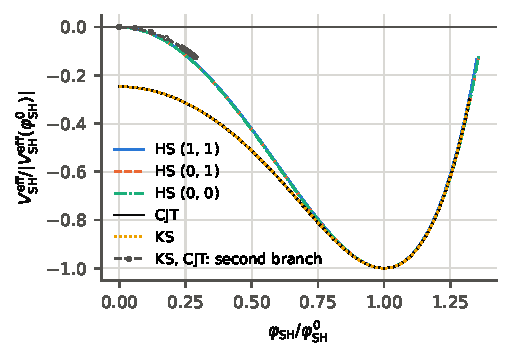
\includegraphics[width=\columnwidth]{figures/fig_prd_sh_potential.pdf}
\caption{The effective potential along the direction of the vacuum, divided by the depth of its minimum, against the
pair amplitude, for the five methods (second version). KS and CJT coincide. The dashed line with circles is the second
branch of KS and CJT, the states continued from the normal vacuum.}
\label{fig:potential}
\end{figure}

\paragraph*{Susceptibilities and masses.}
How does a condensate give a gauge boson a mass? A uniform, static gauge field couples to the densities of the charges,
and its time component acts like a chemical potential $\mu^a=g_aA^a_0$ of the charge $Q_a$. The \emph{susceptibilities}
$\chi^{ab}=\partial\langle Q_a\rangle/\partial\mu^b$ measure how much charge the state takes up in answer. A state with a
gap and no condensate, like the normal vacuum, takes up none, and the gauge bosons stay massless. A condensate answers,
and its answer is its \emph{phase stiffness}, the energy it costs to twist the phase of the condensate from point to
point. In the effective Lagrangian $Z_\SH|D_\mu\Phi|^2$ of the pair fields this stiffness appears as a mass term of the
gauge fields, with the mass matrix
\begin{equation}
(\mathsf M^{\rm g})^2_{ab}=g_ag_b\,\chi^{ab}
\label{eq:Mg}
\end{equation}
on $(W^1_\mu,W^2_\mu,W^3_\mu,B_\mu)$, with $g_a=g$ for $W^a$ and $g'$ for $B$. This is the Higgs mechanism, seen from the
side of the condensate. In the superfluid the susceptibilities are symmetric (by the theorem of Hellmann and Feynman),
the row of the electric charge vanishes in every method, so the photon is massless, and four generators are broken in
the second version (three in the first). In the second version the custodial structure
$\chi(T^a)=\chi(T^a_R)=-\chi(T^a,T^a_R)$ holds, so that the parameter
\begin{equation}
\rho_\SH=\frac{M_W^2}{M_Z^2\cos^2\theta_W}=\frac{\chi^{11}}{\chi^{33}}=1
\label{eq:rho}
\end{equation}
to \ensuremath{2\times10^{-13}} in every method, where $\theta_W$ is the weak mixing angle, $\tan\theta_W=g'/g$. The parameter $\rho$ is
1 at tree level in the Standard Model, a direct consequence of the custodial symmetry of Sec.~\ref{sec:model}. With one
singlet the custodial symmetry is broken and $\rho_\SH$ is \ensuremath{1.202}\mbox{--}\ensuremath{1.247}, which the measured
$M_W^2/(M_Z^2\cos^2\hat\theta_W)=1.0103$~\cite{PDG2026} excludes; the second singlet is what makes the custodial
symmetry exact. In the Standard Model the small departure of the measured value from 1 is a radiative correction, mainly
that of the top quark~\cite{Veltman1977}.

\paragraph*{The scale in GeV.}
From $M_W=\frac12gv_\SH$ the scale is $v_\SH=2(\chi^{11})^{1/2}$, \ensuremath{0.102}\mbox{--}\ensuremath{0.1116} in units of the cutoff (second version,
Table~\ref{tab:masses}). Setting $v_\SH=246.22$~GeV fixes the cutoff at \ensuremath{2207}\mbox{--}\ensuremath{2413}~GeV, and $M_W$ and $M_Z$ take their
measured values. The lightest fermionic excitations, which carry the fractional charges $\frac34$ and $-\frac14$, then
have masses of 848\mbox{--}1093~GeV.

\begin{table*}[t]
\caption{The scale and the masses, second version: $v_\SH$ (units of $\Lambda_\LL$), the cutoff, $\rho_\SH$, and the
amplitude mode from the effective Lagrangian ($M^{\rm EFT}_\SH$, all methods) and from the linear response
($\omega^{\rm H}_\SH$, the pairing-only methods), relative to the scale and in GeV. The Standard Model has
$m_H/v=0.5082$.}
\label{tab:masses}
\begin{ruledtabular}
\begin{tabular}{lccccccc}
method & $v_\SH$ & $\Lambda_\LL$ (GeV) & $\rho_\SH$ & $M^{\rm EFT}_\SH/v_\SH$ & $M^{\rm EFT}_\SH$ (GeV) & $\omega^{\rm H}_\SH/v_\SH$ & $\omega^{\rm H}_\SH$ (GeV)\\
\hline
HS (1,1) & 0.1046 & 2353 & 1 & 9.219 & 2270 & -- & --\\
HS (0,1) & 0.1020 & 2413 & 1 & 9.276 & 2284 & 7.967 & 1962\\
HS (0,0) & 0.1020 & 2413 & 1 & 9.276 & 2284 & 7.967 & 1962\\
KS & 0.1116 & 2207 & 1 & 9.569 & 2356 & -- & --\\
CJT & 0.1116 & 2207 & 1 & 9.569 & 2356 & -- & --\\
\end{tabular}
\end{ruledtabular}
\end{table*}

%=====================================================================================================================
\section{The amplitude mode}
\label{sec:amplitude}

On the Mexican hat a small oscillation of the condensate can go two ways. Along the brim it changes only the phase; this
costs no energy, and these are the Goldstone modes, which in a gauge theory become the longitudinal parts of the massive
gauge bosons. Across the brim it changes the size of the condensate; this costs energy, and the oscillation has a finite
frequency. This second oscillation is the \emph{amplitude mode}. In the Standard Model the Higgs boson is exactly this:
the amplitude mode of the Higgs field. The amplitude mode of our superfluid is therefore the candidate for the Higgs
boson, and its mass is the decisive number. We compute it in two ways.

\paragraph*{Effective Lagrangian.}
At long wavelengths the pair fields obey $Z_\SH(|\partial\Phi^{\rm d}|^2+|\partial\Phi'^{\rm u}|^2)-V^{\rm eff}_\SH$. The
kinetic coefficient follows from the phase stiffness, $\chi^{33}=Z_\SH(\varphi^0_\SH)^2$, and a common oscillation of
the two lengths has the frequency given by the curvature of the potential at its minimum,
\begin{equation}
(M^{\rm EFT}_\SH)^2=\frac{V^{\rm eff\,\prime\prime}_\SH(\varphi^0_\SH)\,(\varphi^0_\SH)^2}{4\chi^{33}} .
\label{eq:MEFT}
\end{equation}
It gives $M^{\rm EFT}_\SH/v_\SH=\ensuremath{9.22}\mbox{--}\ensuremath{9.57}$ in the five methods (Table~\ref{tab:masses}). This formula is the
leading order of an expansion in the frequency, and here the mode lies close to the energy $2E^{\rm gap}$ that breaks a
pair into two quasi-particles (the \emph{threshold}), so the full linear response is needed.

\paragraph*{Linear response.}
The \emph{linear response} describes how the state answers a small, oscillating disturbance of frequency $\omega$; a
natural oscillation of the state shows up as a \emph{pole} of the response, a frequency at which an arbitrarily small
push gives a finite answer. We compute it for the time-dependent mean field at zero momentum, in the sector of relative
number zero, where the fluctuations of the self-energies close under the symmetries of the state. At $\omega=0$ exactly
four singular values of $1-\bm\chi(\omega)\mathsf F$ vanish ($\bm\chi$ the response of the local matrices, $\mathsf F$
the kernel of the contact terms): the four Goldstone modes. In HS (0,1) and HS (0,0), where only the pairing acts, the
response of the pair amplitudes takes the closed form of the theory of Bardeen, Cooper and Schrieffer~\cite{BCS1957}.
With $E=(q^2+M_{\rm eff}^2)^{1/2}$, $M_{\rm eff}^2=m^2+(d^0_\SH)^2/4$, the eigenvalue along the amplitude of the vacuum
direction is
\begin{equation}
\lambda^{\rm amp}(\omega)=\frac{G_\SH}{4\pi^2}\int_0^{\Lambda_\LL}\frac{q^2(q^2+m^2)\,dq}{E\,(E^2-\omega^2/4)} ,
\label{eq:lamamp}
\end{equation}
and the mode is where $\lambda^{\rm amp}(\omega)=1$. With the gap equation $G_\SH I_1(M_{\rm eff})/(4\pi^2)=1$ the identity
\begin{equation}
\lambda^{\rm amp}(\omega)-1=\frac{\omega^2-(d^0_\SH)^2}{4}\,\frac{G_\SH}{4\pi^2}\int_0^{\Lambda_\LL}\frac{q^2\,dq}{E\,(E^2-\omega^2/4)}
\label{eq:identity}
\end{equation}
follows at every momentum. Below the threshold $2M_{\rm eff}$ every term of the integral is positive, so the only zero
is at
\begin{equation}
\omega^{\rm H}_\SH=d^0_\SH ,
\label{eq:omegaH}
\end{equation}
exactly, for every coupling, mass and cutoff: the amplitude mode sits at the pair self-energy. It is a \emph{bound state}
of two quasi-particles, below the threshold by $2M_{\rm eff}-d^0_\SH=0.09309\,\Lambda_\LL$. This is the analogue of the
amplitude mode of a superconductor, which lies at twice the gap parameter, exactly at the
threshold~\cite{LittlewoodVarma1981,PekkerVarma2015}; here the mass of the fields raises the threshold above the mode. The Rust program, which solves the
full response of the sector and does not use (\ref{eq:lamamp}), finds (\ref{eq:omegaH}) to \ensuremath{2\times10^{-13}}; the Python
program confirms (\ref{eq:lamamp}) numerically, and the Wolfram script derives (\ref{eq:identity}) symbolically. With the
scale of the second version, $M_H/v_\SH=7.967$, that is $M_H=1962$~GeV, against the measured
$m_H/v=0.5082$: the amplitude mode is 16 times too heavy relative to the scale.

\paragraph*{No coupling repairs it.}
In HS (0,0) the ground state has a closed form, so the ratio can be followed over the coupling. For
$1.02\le G_\SH/G^{\rm crit}_\SH\le3$ and the masses $0.1$ and $0.2$ of the fields it lies between \ensuremath{4.892} and
\ensuremath{34.43} in the second version (Fig.~\ref{fig:scan}), where $\rho_\SH=1$ at every point. The ratio is smallest near
the critical coupling, where $d^0_\SH$ and $v_\SH$ both vanish, and it grows with the coupling, because $d^0_\SH$ grows
while $v_\SH$, limited by the cutoff, stays below 0.14. Even its smallest value is 9.6 times the
measured $m_H/v$.

\begin{figure}[t]
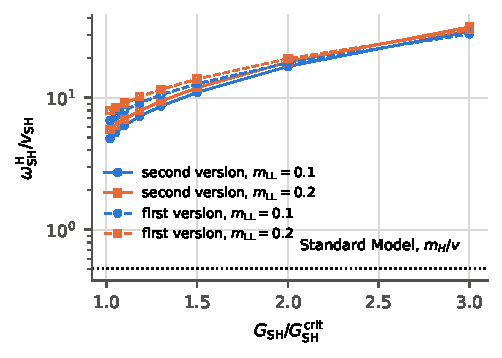
\includegraphics[width=\columnwidth]{figures/fig_prd_sh_scan.pdf}
\caption{The ratio of the mass of the amplitude mode to the scale, $\omega^{\rm H}_\SH/v_\SH$, against the coupling, in
HS (0,0) for the masses 0.1 and 0.2 of the fields, in both versions, with the measured $m_H/v$.}
\label{fig:scan}
\end{figure}

\paragraph*{The partners of the amplitude mode.}
The bidoublet has eight real components, so there are eight small oscillations. In HS (0,0) four lie at $\omega=0$ and
four at $\omega=d^0_\SH$. The custodial group $SU(2)_V$ commutes with the response and sorts each set of four into a singlet
and a triplet. At $\omega=0$ the triplet becomes the longitudinal parts of $W^\pm$ and $Z$, and the singlet is the
Goldstone boson of the particle number, a massless neutral scalar that the model has to remove, by gauging
$F^{\rm tot}_\SH$ or by breaking it explicitly; this is left open here. At $\omega=d^0_\SH$ the singlet is the candidate
for the Higgs boson, and the triplet holds a neutral scalar and a charged scalar with its antiparticle, degenerate with it
in the pairing-only methods. Together they are the scalar content of two Higgs doublets.

%=====================================================================================================================
\section{Dynamics in time}
\label{sec:dynamics}

The linear response predicts frequencies; the \emph{time-dependent mean field}, in which the averages of the state evolve
by the equations of motion of the quasi-particles, shows them as motion. We integrate it for each method with CVODE
(relative tolerance $10^{-12}$). The energy, the charges of the symmetries and the orthonormality of the quasi-particle
vectors are conserved to the accuracy of the integration, and the ground state stays at rest, as it must. A small
displacement of the pair fields along the vacuum direction (a push across the brim of the hat) oscillates, in HS (0,1)
and HS (0,0), at $d^0_\SH$ to \ensuremath{2\times10^{-6}}, without damping, in both versions; a displacement along the custodial
triplet oscillates at the same frequency. In HS (1,1) the mode lies at 0.9736\,$d^0_\SH$, below the energy
that breaks a pair, and is undamped; the scalar and the vector terms raise the triplet by 2.2 per cent. In KS
and CJT the spectrum peaks at 0.873546\,$\Lambda_\LL$, above the threshold 0.768402\,$\Lambda_\LL$, with a width
1.8 times that of an undamped oscillation of the same length: there the amplitude mode decays into pairs of
quasi-particles, a \emph{resonance} rather than a bound state (Fig.~\ref{fig:modes}). With a chemical potential $\mu$ of the
particle number the phase of the pair fields turns at the rate $2\mu$ (the Josephson relation: a pair carries the
particle number 2), to \ensuremath{2\times10^{-9}}. A displacement by 30 per cent in HS (0,0) oscillates at 0.9582\,$d^0_\SH$:
the oscillation softens with its amplitude, as a ball rolling higher on the walls of a Mexican hat would.

\begin{figure}[t]
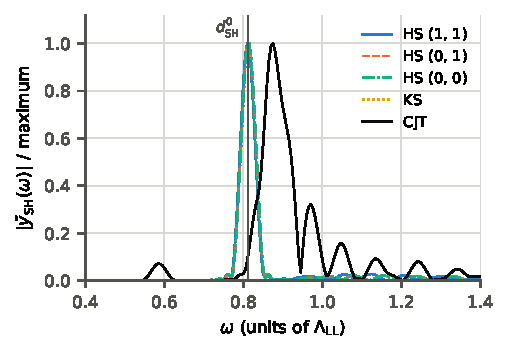
\includegraphics[width=\columnwidth]{figures/fig_prd_sh_modes.pdf}
\caption{The spectra of the length $|d(t)|$ of the pair self-energy after a small displacement along the vacuum
direction, second version, each divided by its largest value; $d^0_\SH$ of the pairing-only methods is marked. KS and
CJT coincide.}
\label{fig:modes}
\end{figure}

%=====================================================================================================================
\section{Can the superfluid be the Higgs field of the Standard Model?}
\label{sec:higgs}

\paragraph*{What works.}
The superfluid of the second version has the quantum numbers of the Higgs field, breaks $SU(2)_L\times U(1)_Y$ to the
$U(1)$ of the electric charge, keeps the photon massless and gives $\rho_\SH=1$. With the scale set to $v$, the $W$ and
$Z$ bosons have the masses of the Standard Model at tree level. These are consequences of the quantum numbers and of the
custodial vacuum, and they hold in all five methods.

\paragraph*{What fails.}
The amplitude mode is \ensuremath{16}\mbox{--}\ensuremath{19} times too heavy relative to the scale (16 times from the linear
response, 18\mbox{--}19 times from the effective Lagrangian). The reason is simple. In a superfluid of fermion pairs
bound by a contact interaction, the amplitude mode lies at $d^0_\SH$, just below the energy $2M_{\rm eff}$ that breaks a
pair, while $v_\SH^2$, the phase stiffness, grows only like $M_{\rm eff}^2$ times the logarithm of
$\Lambda_\LL^2/M_{\rm eff}^2$ (in the leading approximation, divided by $4\pi^2$ and multiplied by the number of paired
species). Here the cutoff is only about twice $M_{\rm eff}$, so the logarithm is small, $v_\SH$ is small compared with
$M_{\rm eff}$, and the ratio $M_H/v_\SH$ is large. The same relation underlies the models in which the Higgs doublet is a
bound state of the top quark and its antiparticle, where a light Higgs boson needs a very high cutoff~\cite{BHL1990}.

\paragraph*{What the model adds.}
The second doublet brings a custodial triplet of massive scalars, degenerate with the candidate in the pairing-only
methods and split from it by 2.2 per cent in HS (1,1); the particle number brings a massless Goldstone
boson; and the constituents are fermions with the fractional electric charges $\frac34$ and $-\frac14$ and masses of
848\mbox{--}1093~GeV. Each of these must be confronted with experiment before the model can be compared with the
observed Higgs sector.

\paragraph*{What remains open.}
The mean field leaves out the fluctuations of the pair fields, which shift both the stiffness and the amplitude mode; a
computation beyond it is needed before the ratio $M_H/v$ can be called a prediction of the model. The thermal transition
of the revised model has not been computed either, so the width of its \emph{critical region}, the range of temperatures
near the transition in which the fluctuations of the order parameter, which the mean field leaves out, dominate (as
measured by the criterion of Levanyuk and Ginzburg~\cite{Levanyuk1959,Ginzburg1960}), is not known here.

%=====================================================================================================================
\section{Is the Higgs a composite particle?}
\label{sec:composite}

A particle is \emph{composite} if it is a bound state or a resonance of more elementary constituents, as a hydrogen atom
is of a proton and an electron. In this model there is no elementary scalar field at all: the order parameter of the
Higgs field is the expectation value of the pair operators, a composite of a member of $\Psi_\LL$ and a singlet. The
amplitude mode is a bound state of two quasi-particles below the threshold that breaks a pair in HS (0,1), HS (0,0) and HS
(1,1), and a resonance above it, decaying into pairs, in KS and CJT. The Higgs particle of the model is therefore
composite by construction, and whether it is a sharp state depends on the method; in none of them is it light enough to
be the observed Higgs boson.

%=====================================================================================================================
\section{Toward the gravitational sector}
\label{sec:gravity}

The factor $SL(2,\mathbb C)$ of the gauge group acts on the spinor indices of all three fields with the Lorentz connection
$\Gamma^\LL_\mu$ of (\ref{eq:cov}), which on flat M31 is a pure gauge. Lord~\cite{Lord1971} considered the group of
changes of representation of the two-component spinor algebra, under which the free field equations of particles of any
spin are invariant, and made it a gauge group in the sense of Yang and Mills. Gauge invariance and Lorentz covariance
then require auxiliary fields; Lord interpreted them as the potentials of a field of spin two, which is then
self-interacting, and showed that the Bargmann-Wigner equations of the linear spin-two field (its field equations
written as one Dirac equation for each of its spinor indices), modified by this self-interaction, give a nonlinear theory
identical with Einstein's. This construction is the natural route for the
present model because its spinor charges come with $SL(2,\mathbb C)$ from the super-loop (Sec.~\ref{sec:lorentz}). The
program is (i) to replace the pure-gauge $\Gamma^\LL_\mu$ by Lord's gauge field and its auxiliary fields, (ii) to couple
the spinor fields and their pairs to it, and (iii) to obtain the gravitational field equations with the
energy-momentum tensor of the spinor fields as their source. Gauging the local Lorentz group is also the route of Utiyama
and Kibble~\cite{Utiyama1956,Kibble1961,Hehl1976}. The superfluid is a Lorentz scalar and leaves $SL(2,\mathbb C)$
unbroken, so the condensation does not give the gravitational field a mass. The quantization of the gravitational sector,
and with it the ``quantum gravity'' of the title, is beyond this paper.

%=====================================================================================================================
\section{Conclusions}
\label{sec:conclusions}

The bi-octonions of unit norm form a Moufang loop that contains the Lorentz group and eight spinor charges, carried by
an isodoublet of Dirac spinors. Pairs of two members of that isodoublet are isospin triplets, so their superfluid cannot
be the Higgs field. Two singlet Dirac fields with the hypercharges $\frac14$ and $-\frac34$ change this: the superfluid of
pairs of the isodoublet with a singlet is a composite with the quantum numbers of two Higgs doublets. In five mean-field
methods its ground state is the custodial vacuum, which breaks the electroweak group to electromagnetism, gives $\rho=1$,
and, with its scale set to $v$, gives the $W$ and $Z$ bosons their masses. Its amplitude mode, a composite scalar, lies
exactly at the pair self-energy in the methods in which only the pairing acts, and is about sixteen times too heavy
relative to the scale, because the phase stiffness of a superfluid bound by a contact interaction below a low cutoff is
small. The model therefore reproduces the Higgs field of the Standard Model in its quantum numbers and its gauge-boson
masses, but, in the mean field, not in the mass of its boson. The gravitational sector will be added through Lord's gauge
theory of the local change of spinor representation, for which the model already has the place.

%=====================================================================================================================
\section*{Data availability}

The data that support the findings of this article are openly available in the repository of PROJECT
spacetimes~\cite{Repo}, folder \texttt{Revision\_SM\_Higgs}: the data files (\texttt{data/}), the Rust, Python and Wolfram
Language programs that produce and check them (\texttt{rust/}, \texttt{python/}, \texttt{wolfram/}), the reports of their
checks, the notebook, and the scripts that build this article from the data (\texttt{paper\_prd/}). The Supplemental
Material~\cite{SM} lists the files with their SHA-256 checksums.

\begin{acknowledgments}
The computations used the SUNDIALS integrators in a Rust implementation, numpy and LAPACK.
\end{acknowledgments}

\bibliography{references}

\end{document}
